%-----------------------------------------------------------------------------
% CONFIGURE DOCUMENT
%-----------------------------------------------------------------------------

%\documentclass[letterpaper, 10 pt, conference]{ieeeconf}  % Comment this line out
                                                           % if you need a4paper
\documentclass[letterpaper, 12pt, conference]{ieeeconf}    % Use this line for a4
                                                           % paper

\IEEEoverridecommandlockouts                              % This command is only
                                                          % needed if you want to
                                                          % use the \thanks command 
\overrideIEEEmargins
% See the \addtolength command later in the file to balance the column lengths
% on the last page of the document
% The following packages can be found on http:\\www.ctan.org

%\smartqed  % flush right qed marks, e.g. at end of proof
%
% The following packages can be found on http:\\www.ctan.org
\usepackage{graphics} % for pdf, bitmapped graphics files
%\usepackage{epsfig} % for postscript graphics files
%\usepackage{mathptmx} % assumes new font selection scheme installed
%\usepackage{times} % assumes new font selection scheme installed
\usepackage{amsmath} % assumes amsmath package installed
\usepackage{amssymb}  % assumes amsmath package installed
\usepackage{url}
    % By default the URLs are put in typewriter type in the body and the
    % bibliography of the document when using the \url command.  If you are
    % using many long URLs you may want to uncommennt the next line so they
    % are typeset a little smaller.
\renewcommand{\UrlFont}{\small\tt}
\usepackage{graphicx}
\usepackage{listings}
\usepackage{color}
\usepackage[tight]{subfigure}
%\usepackage{tabu}
%\usepackage{algorithm}
%\usepackage{algorithmic}
\usepackage{balance}
\usepackage[ruled,vlined]{algorithm2e}

\usepackage{listings}
  \usepackage{courier}
 \lstset{
         %basicstyle=\footnotesize\ttfamily, % Standardschrift
         basicstyle=\scriptsize\ttfamily, % Standardschrift
         %numbers=left,               % Ort der Zeilennummern
         numberstyle=\tiny,          % Stil der Zeilennummern
         %stepnumber=2,               % Abstand zwischen den Zeilennummern
         numbersep=5pt,              % Abstand der Nummern zum Text
         tabsize=1,                  % Groesse von Tabs
         extendedchars=true,         %
         breaklines=true,            % Zeilen werden Umgebrochen
         keywordstyle=\color{red},
            frame=b,
 %        keywordstyle=[1]\textbf,    % Stil der Keywords
 %        keywordstyle=[2]\textbf,    %
 %        keywordstyle=[3]\textbf,    %
 %        keywordstyle=[4]\textbf,   \sqrt{\sqrt{}} %
         stringstyle=\color{white}\ttfamily, % Farbe der String
         showspaces=false,           % Leerzeichen anzeigen ?
         showtabs=false,             % Tabs anzeigen ?
         xleftmargin=17pt,
         framexleftmargin=17pt,
         framexrightmargin=5pt,
         framexbottommargin=4pt,
         %backgroundcolor=\color{lightgray},
         showstringspaces=false      % Leerzeichen in Strings anzeigen ?
 }
 \lstloadlanguages{% Check Dokumentation for further languages ...
         %[Visual]Basic
         %Pascal
         %C
         %C++
         XML
         %HTML
         %Java
 }
    %\DeclareCaptionFont{blue}{\color{blue}}

  %\captionsetup[lstlisting]{singlelinecheck=false, labelfont={blue}, textfont={blue}}
  \usepackage{caption}
    %\DeclareCaptionFont{white}{\color{white}}
    %\DeclareCaptionFormat{listing}{\colorbox[cmyk]{0.43, 0.35,0.35,0.01}{\parbox{\textwidth}{\hspace{15pt}#1#2#3}}}
    \DeclareCaptionFormat{listing}{\colorbox[cmyk]{0, 0,0,0}{\parbox{\columnwidth}{\hspace{15pt}#1#2#3}}}
    %\captionsetup[lstlisting]{format=listing,labelfont=white,textfont=white,singlelinecheck=false, margin=0pt, font={bf,footnotesize}}
    \captionsetup[lstlisting]{format=listing,singlelinecheck=false, margin=0pt}

\graphicspath{{./}{./figures/}}

%-----------------------------------------------------------------------------
% TITLE
%-----------------------------------------------------------------------------

\title{\LARGE \bf Planning engine driven by task allocation and symbolic planners for multi-UAV assembly missions optimization}

%-----------------------------------------------------------------------------
% AUTHORS and CONTACTS
%-----------------------------------------------------------------------------

\author{Jorge Munoz-Morera, Ivan Maza, \\ Fernando Caballero and Anibal Ollero   % $<$-this % stops a space
\thanks{This work has been partially supported by the ARCAS Project (FP7-ICT-287617) funded by the EU FP7 and the RANCOM Project (P11-TIC-7066)} % $<$-this % stops a space
\thanks{Robotics, Vision and Control Group, University of Seville, Avd. de los Descubrimientos s/n, 41092, Sevilla, Spain. Email:
{\tt\small jorgemunoz@us.es, imaza@us.es, fcaballero@us.es, aollero@us.es}}
}

%-----------------------------------------------------------------------------
% DOCUMENT
%-----------------------------------------------------------------------------
\begin{document}

\maketitle

\thispagestyle{empty}

\pagestyle{empty}

%-----------------------------------------------------------------------------
% ABSTRACT
%-----------------------------------------------------------------------------
\begin{abstract}
The work presented in this paper is part of the autonomous planning architecture of a team of aerial robots equipped with on-board robotic arms. The mission of the team is the construction of structures in places where the access is difficult by conventional means, which is the scenario considered in the framework of the ARCAS European Project. This paper presents a planning engine for this context. From the 3D CAD model of the structure an assembly planner computes the required assembly operations, which are the inputs for the system. These operations are assigned to the available aerial robots by a task allocation planner, which computes an assignment and optimizes it by communicating with a symbolic planner that estimates the cost of the sequence of actions needed in the mission execution for the given assignment. This paper centers on plan optimization and includes benchmarking and simulation results that show the feasibility of the approach and the properties of the solutions.  
\end{abstract}
 
%-----------------------------------------------------------------------------
% KEYWORDS
%-----------------------------------------------------------------------------

\begin{keywords}
Assembly Planning; Symbolic Planning; Task Planning; Task Allocation; Multiple UAS
\end{keywords}

\section{Introduction and Related Work}
\label{sec:intro}

The work described in this paper is part of the ARCAS European Project~\cite{kondak_ijars13} funded by the European Commission. One of the goals of this project is to build a structure by using a team of aerial robots equipped with on-board manipulators. The practical interest of this system can be found in situations where it is required to build a structure in places with difficult access by conventional means.

% (see Fig.~\ref{fig:arcas}).

%\begin{figure}
%\centerline{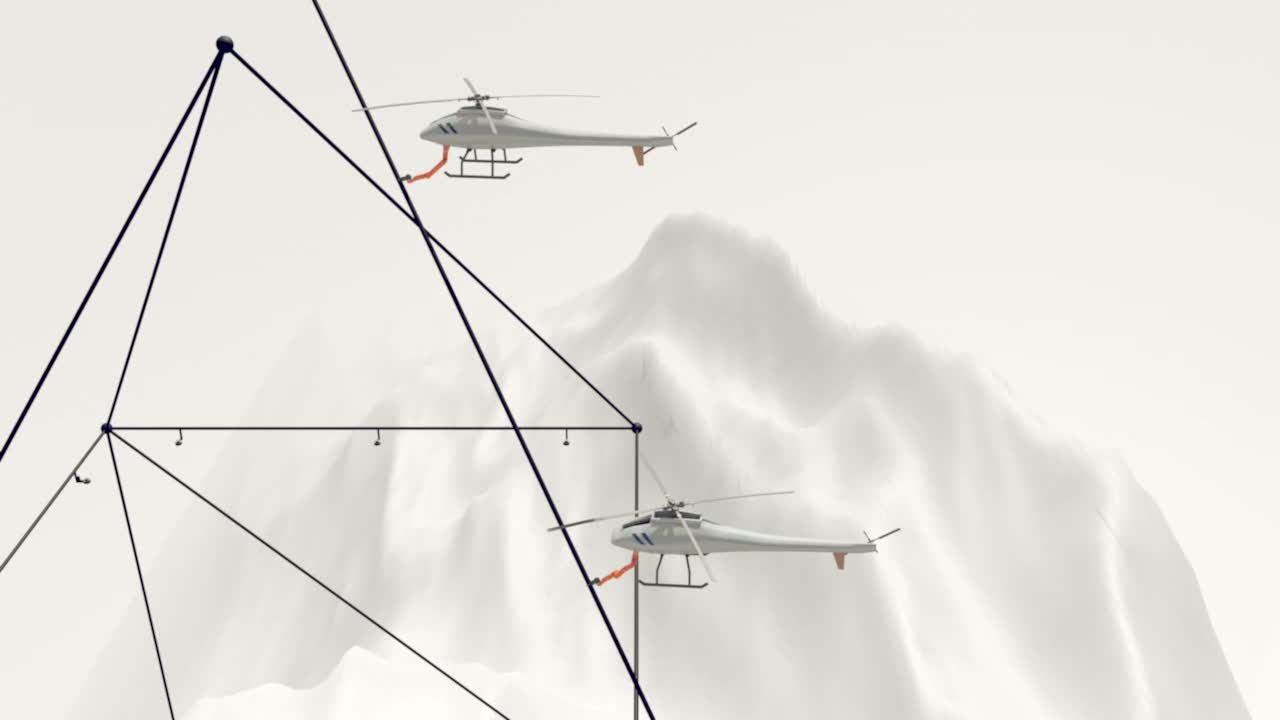
\includegraphics[width=0.99\columnwidth]{arcas.jpg}}
% \caption{Two aerial robots equipped with LWR KUKA robotic arms manipulating a bar to build a structure in places with difficult access by conventional means.}
% \label{fig:arcas}
%\end{figure}

Although Unmanned Aerial Systems (UAS) have been designed and developed for performing military missions, currently the trend is to extend their applicability to civil mission such as firefighting, critical infrastructure protection or remote surveillance, among many others.  The multiple variety of platforms, control systems and ground-based equipments~\cite{perez_jint13,maza_jint10_multimodal}, and the heterogeneity of the communication devices have made difficult the interoperability among different systems. 

Several works~\cite{maza_icuas14,maza_jfr11_multiuav} have addressed cooperation in teams of aerial robots for multi-purpose missions. However, in those papers the dexterous manipulation with aerial robots was not present. The use of aerial robots allows to perform assembly operations in any point of the 3D space, which can represent a relevant advantage compared to ground robots in areas of difficult access. Assembly planning is the process of creating a detailed assembly plan to craft a whole product from separate parts by taking into account the final product geometry, available resources to manufacture that product, fixture design, feeder and tool descriptions, etc. Efficient assembly plans can reduce time and costs significantly. The assembly planning problem has been shown to be an NP-complete problem~\cite{Kavraki93} and covers three main assembly subproblems: sequence planning, line balancing, and path planning. Reference~\cite{Jimenez2011} presents a survey on assembly sequencing from a combinatorial and geometrical perspective.

Most existing classical planners can be classified into two categories~\cite{ingrand_ghallab_2013}: planners which use domain-dependent knowledge and planners which use domain-independent knowledge. The former can exploit their specific knowledge to guide the planning process and solve larger problems faster than other planners, with the disadvantage of needing a person who gives the knowledge on how to solve the problems. Such knowledge can be designed using temporal logic (TLPlan~\cite{Bacchus00usingtemporal} and TALplanner~\cite{Kvarnstrom01talplanner}) or task decomposition (SHOP2~\cite{Nau03shop2}, SIPE-2~\cite{Wilkins}, O-PLAN~\cite{Currie90}). On the other hand, a planner that uses domain-independent knowledge (SGPlan~\cite{Chen06}, FastDownward~\cite{Helmert06}, LPG~\cite{Gerevini01}) does not need specific knowledge so the domain formalization is simpler, with the disadvantage that the performance of the planner may be lower than that of domain-dependent planners. The integration of both types of planners, which let use their advantages and avoid their disadvantages, is a matter of study, and some works in that direction can be read in~\cite{Gerevini02} and~\cite{Shivashankar}.

Below the task planning is situated the motion and manipulation planning, which should take into account the geometry, kinematics and dynamics of the problem. For motion planning there are consolidated techniques which produce very good results, such these based on Rapidly-exploring Random Trees~\cite{LaValle04}. Combined task and motion planning have been studied in different works~\cite{Cambon01012009,Wolfe,Lagriffoul01122014}, but this work only addresses up to task planning. A system on which teams of quadrotors assemble a 2.5-D structure from simple parts can be found in~\cite{Lindsey-RSS-11}. In that work the robots were equipped with grippers and the structure was supposed to be assembled sequentially, so no manipulation planning was done after picking the parts and the assembly operations were not parallelizable.

This paper presents a planning engine to solve a general structure assembly problem with a team of UAS. From the 3D CAD model of the structure the assembly planner presented in Sect.~\ref{sec:assembly_sequence} computes the required assembly operations, which are the inputs for the system. These operations are assigned to the available aerial robots by the task allocation planner described in Sect.~\ref{sec:ata}. This planner optimizes the computed assignment by communicating with the symbolic planner explained in Sect.~\ref{sec:ats}, which estimates the cost of the sequence of actions needed in the mission execution for the given assignment and gives feedback to the task allocation planner in the search of a better assignment. This paper centers on plan optimization and includes benchmarking and simulation results in Sect.~\ref{sec:results} that show the feasibility of the approach and the properties of the solutions. Section~\ref{sec:conclusions} closes the paper with the conclusions and future work.

%. One approximation to connect the task planning level and the motion planning level is the use of a top-down model: the high level provides the low level with a planning instance, and the low level returns a single solution or fails if it is unfeasible. By this way, most unfeasible plans are rejected at the task planning level, while the motion planning level is used only when the refining of the high level plan is needed. One planner that merges the capabilities of symbolic and geometric planners is aSyMov~\cite{Cambon01012009}, a task planner that takes into account the geometrical and topological constraints of the geometrical environment and that tries to fit the gap between the symbolic representation and its geometric counterpart to solve robotics problems where the motion and manipulation planning is needed. Another example of task and motion planning integration can be viewed in \cite{Wolfe}, where a hierarchical planning system is applied to manipulation robotics. In the system, the primitive actions responsible of the robot's base or arm movements are modelled with calls to external solvers based on RRTs. Continuous choices such as grasp angles are made finite via sampling while the sensorial data and robustness to failures are managed inside the primitive actions. Although combined task and motion planning works well with real robotics problems, one disadvantage is that the task planner generates initially feasible high-level plans in the symbolic level that may turn into unfeasible when evaluated at the geometric level, which is traduced in a waste of significant computational effort. A work that dives into that problem can be found in~\cite{Lagriffoul01122014}, where an intermediate layer between the task planning and the geometric reasoning consisting on a constraint network is proposed to prune the search space during the geometric evaluation of the symbolic action sequences.

\section{Assembly Planner}
	\label{sec:assembly_sequence}

From the 3D CAD model of the structure, a framework for assembly planning has been developed taking into account the physical stability of the partial substructures in the presence of the external force of the gravity. The assembly planner is composed by a classical planner, a simulation engine based on the Bullet Physics library~\cite{bullet} and a visualization component that is provided as an optional tool. 

The purpose of the assembly planner is to obtain an assembly plan with all the assembly operations needed to build the structure from an initial state where no part is assembled to a final state where all parts are assembled, given by the 3D CAD model itself. The assembly plan is computed by using the \emph{assembly-by-disassembly} technique, consisting on finding a plan to disassemble the whole structure and reversing the order of its operations to get the final assembly plan.

The output of the assembly planner is an XML file containing the assembly operations. Each operation represents the assembly of one specific part of the structure and contains the preconditions that must be met prior to its execution, namely the assembly operations that must be done before the assembly of that specific part. In the output plan file the assembly operations are partially ordered, meaning that the assembly could be correctly done by doing the operations in appereance order, but operations that appear later in the file may be executed in parallel or even before some of the previous.

\section{Tasks Assignment in a multi-UAS context}
\label{sec:ata}

After the generation of a plan composed of assembly tasks, the next step is the generation of an initial assignment of these tasks to the available UAS. This section contains the problem definition and the details of the planner that solves it.
    
Let us consider a mission $\mathcal{M}$ consisting on the assembly of a structure composed by several parts initially located around the environment. The parts have to be assembled on specific locations by a team of $n$ UAS starting the mission from their home locations. Then the mission is composed by a set of assembly tasks $\mathcal{T}$. Each of the parts has a weight and a dependency list consisting on the tasks that must be done prior to its assembly. Let us define $\mathcal{L}$ as the set of stock parts locations, $\mathcal{L'}$ as the set of locations where the parts have to be assembled and $\mathcal{H}$ as the home locations of the UAS. The objective is to assemble all the parts on their locations minimizing the travel flight times of the vehicles and exploiting the potential parallelism that can be achieved using multiple UAS.
    
The implicit combinatorial problem can be expressed by the edges of a graph $G(V,E)$ considering the following notation:
    
    \begin{itemize}
    	\item $\mathcal{T} = \{t_1, t_2, ..., t_m\}$ is a set of $m$ assembly tasks.
    	\item $n$ is the number of UAS.
    	\item $\mathcal{L} = \{l_1, l_2, ..., l_m\}$ is the set of stock parts locations and $\mathcal{L'} = \{l'_1, l'_2, ..., l'_m\}$ is the set of final assembly locations.    
    	\item $\mathcal{H} = \{h_1, h_2, ..., h_n\}$ is the set of UAS home locations.
  		\item $V=\{\mathcal{L}\cup\mathcal{L'}\cup\mathcal{H}\}=\{v_1, v_2, ..., v_{2m+n}\}$ is the set of vertices of the $G$ graph.
		\item $E=\{(v_i,v_j) | v_i,v_j \in V; i<j\}$ is the edge set.  		
  		\item ${R_{k} = \{r_1, r_2, ..., r_s} \}\subseteq$ $V$ is the route for the $k$-th UAS, composed by a subset of $s$ vertices from $V$.
		\item Cost $c_{r_i,r_j}$ is a non-negative travel time between vertex $r_i$ and $r_j$, where $c_{r_i,r_j}=c_{r_j,r_i}$.
		\item $w = \{w_1, w_2, ..., w_m\}$ is a vector containing the weights of the parts.	
		\item $p = \{p_1, p_2, ..., p_n\}$ is a vector with the maximum payloads of the UAS.
	\end{itemize}
	
	The problem consists in determining a set $\mathcal{R}$ of UAS routes with minimal cost, each starting at the home locations of the vehicles, such that every vertex in $\mathcal{L}$ is visited at least by one vehicle and followed by its subsequent vertex in $\mathcal{L'}$, without exceeding the payload of each vehicle. The possibility of visiting the same location with multiple UAS is given by the fact that some parts should be carried cooperatively by more than one UAS if they are too heavy. The problem described is similar to the well-known Vehicle Routing Problem (VRP)~\cite{Dantzig_Ramser_VRP}.	
	For the $k$-th UAS, the cost of a route is given by 

 \begin{equation}
 	{C(R_{k}) = \sum_{i=1}^{s-1} c_{r_i,r_{i+1}}} \, ,
 	\label{eq:route_cost}
 \end{equation}	

\noindent where ${r_1 \in \mathcal{H}}$, ${r_i \in V}$ and ${r_j \in}$ $\mathcal{L}$ ${\implies r_{j+1} \in}$ $\mathcal{L'}$. Considering that up to two UAS can cooperatively transport a single heavy part, this route ${R_{k}}$ is feasible if ${(p_k \geq w_j) \lor (\exists R_{z} | r_j \in R_{z} \land (p_k+p_z) \geq w_j)}$, i.e. the weight of each part does not exceed the maximum payload of the UAS transporting it or there is another available UAS so that both can transport it cooperatively.
	
On the other hand, a score has been defined for each solution in order to balance the workload of the different UAS. This score consists on a numerical value that is increased as a penalty whenever the task allocation for each UAS diverges from the allocation where all the UAS have the same number of tasks allocated.
	
The goal of the planner is to minimize the total travel time $\sum_{i=1}^{n} C(R_{i})$ of the feasible routes executing all the assembly tasks of the mission, and minimizing also the score mentioned above.
    
The planner chosen to solve the assignment problem presented in this section was OptaPlanner~\cite{optaplanner}, an open source, multi-platform planning engine written in Java and released under Apache Software License. OptaPlanner is aimed to solve planning problems with resource usage optimization. It is capable of generating near-optimal plans by applying optimization heuristics and meta-heuristics combined with score calculation. One of his main advantages is that the solver's algorithm is highly configurable. In OptaPlanner it is possible to use different heuristics and meta-heuristics algorithms applied in sequence, so that the user can select the most suitable for the problem in question. The optimization is done in base of a score calculation that is computed after all the planning entities have been assigned. This score determines the suitability of the last computed solution: if after searching for a new solution, the new score is higher than the score calculated in the previous solution, then the last solution is discarded and the process continues trying to generate a solution with a lower score.

%As it was mentioned above, the OptaPlanner solver can use multiple optimization algorithms in sequence. Each of the optimization algorithms used is called a solver phase. During the execution of the solver there is never more than one solver phase executing at the same time, so a solver phase only starts when the previous phase has finished. There are three types of solver phases that can be used in the OptaPlanner solver: Construction Heuristics (CH), Metaheuristics (MH) and Exhaustive Search (ES). 

%The CH solver phase builds an initial solution in finite time. The solution computed is not always feasible, but it tries to find it fast so that the following solver phases can finish the searching of a feasible one by starting from that initial solution. There are different algorithms that can be used as CH. One common characteristic of them is that when a CH assigns a planning variable, that assignment remains unchanged until the end of the algorithm. This is the main reason that makes the CH algorithms find solutions that may be unfeasible: no re-planning is done at this phase.
%
%The MH phase is based on different types of local search algorithms. Local search starts from the initial solution computed by the CH phase and evolves that into a mostly better and better solution. At each solution, it evaluates a number of moves between the planning entities of the solution and applies the most suitable to step to the next solution, whose score has to be equal or better (lower) than the previous. One important thing to be taken into account is that the local search does not use a search tree, but a search path. When finding a new solution all possible moves are tried but unless it is the chosen move, it does not investigate further the rest of possible solutions. That makes the local search very scalable, but as a disadvantage it may not find never the optimal solution.
%
%The last ES solver phase does not depend on previous phases and it is applied alone. Brute force or the branch and bound algorithms are available. These methods can find the optimal solution for a problem, but are poorly scalable.

It should be mentioned that one task may be required to be executed by more than a single UAS. In order to do so, certain tasks are automatically divided and the workload is shared. This is the case of heavy parts that could not be carried by a single UAS. The associated assembly task is divided in several assembly tasks with less weight that can be executed by several cooperative UAS.

%On the other hand, the constraints mentioned above have been modelled by using a hard/medium/soft score within OptaPlanner. %

%This type of score define three types of constraints with different levels of relevance:
%
%    \begin{itemize}
%    	\item Hard-constraints: these are constraints that must not be broken in any case. A broken hard-constraint will lead to an unfeasible plan. The hard-constraints defined for the problem say that a discretized task must be assigned to different UAS and that the base and roof parts of the structure must be assigned in a balanced way among the UAS.
%    	\item Medium-constraints: these are constraints that are desirable to be broken the less as possible. Its importance is under the importance of the hard-constraints but above the importance of the soft-constraints. The one defined states that given a part with dependencies, all of its dependencies must be assigned to as different UAS as possible.
%    	\item Soft-constraints: these are the constraints with lower priority. They have the lowest impact when broken, but still they must be minimized. The soft-constraint defined tries to minimize the distance travelled by all the UAS.
%	\end{itemize}

\section{Assembly Tasks Sequencing}
	\label{sec:ats}

Up to this point, the assembly plan contains the sequence of assembly tasks that are needed to consistently build the structure. Some of the tasks in the computed plan could be executed in parallel to reduce the whole mission assembly time. This information is implicitly encoded in the plan as task preconditions. Each assembly task has a list associated containing all the preconditions that must be met in order to be able to perform the operation. At any given instant, all the assembly tasks that have their preconditions met, could be executed in parallel. 

%Thus, the assembly tasks computed by the assembly planner can be ordered in time to reduce the assembly time and maximize the parallelism among the task executions.

In addition to the minimization of the assembly time, a low level plan must be computed for each UAS. Feasible paths must be computed for the navigation of the robots, both for the part picking and the part assembling. Also, those assembly tasks that must be executed cooperatively between robots require the synchronization among the involved UAS.

%This section presents an overview of the planner, giving some details of its fundamentals. The planning domain designed for the JSHOP2 planner is also described.

%\subsection{JSHOP2 Overview}
%    \label{sec:shop2ov}

In this paper, the JSHOP2 symbolic planner~\cite{Nau03shop2} has been applied to order the assembly tasks as well as to compute a low level plan for each UAS. JSHOP2 is a domain-independent planning system based on Hierarchical Task Network (HTN) that decomposes the tasks into subtasks, then the subtasks into smaller subtasks and so on, until obtaining low-level tasks that can not be further decomposed and thus can be directly performed. These low-level tasks are called primitive tasks.

The inputs to JSHOP2 are a planning domain and a planning problem. The planning domains are composed of methods, operators and axioms, while the planning problems are composed of logical atoms and task lists. The methods, operators and axioms that compose a planning domain all involve logical expressions that combine logical atoms. The logical atoms conform the initial state of the problem, and the task lists represent the high-level actions that must be performed (the goals) by decomposing them into lower-level actions called primitives. The decomposition is done by the use of methods, which decompose the high level tasks into smaller ones until obtaining the primitives, which are represented by the operators.

%The main components of a JSHOP2 planning domain/problem are the following:
%
%\begin{itemize}
%  \item Tasks: a task represent an activity to perform. Tasks can be of two different types: primitive or compound. A primitive is a low-level task that can not be further decomposed and that can be accomplished immediately by a planning operator. A compound task is one that must be decomposed into several smaller subtasks by using methods and/or operators.
%  \item Operators: the operators tell how a primitive task can be performed. Each operator has a precondition expression composed of logical atoms that must be true in the current state for the operator in order to be applicable. Also, a \textit{delete list} and \textit{add list} are present giving the negative and positive effects that are consequence of applying the operator.
%  \item Methods: the methods tell how a compound task must be decomposed into an ordered set of subtasks, where each can be also a compound task or a primitive task. A method is composed of preconditions that must be satisfied in the current state for the method in order to be applicable, and the subtasks on which the method is decomposed and that must also be accomplished. A method can have more than one pair preconditions-subtasks, which are evaluated in order of appearance.
%  \item Axioms: axioms are constructs that can be used to infer preconditions that are not explicitly asserted in the given state.
%  \item External function calls: in JSHOP2 it is possible to make external Java function calls from the preconditions of a method. These calls allow the execution of external code or libraries to run calculations or evaluations that in other ways could not be done from inside the JSHOP2 planning engine.
%\end{itemize}

%One of the main characteristics of JSHOP2 is that it plans for tasks in the same order that they will be executed. The input for JSHOP2
%is a problem file that contains a partially ordered set of tasks. The tasks appear in sequence so JSHOP2 will plan for them in that order. However it is possible that the execution of the tasks in the resulting plan does not follow that order strictly. This feature was used in the domain description for our specific problem and will be explained with greater detail in the following.

The format of the problem and domain files in JSHOP2 is very similar to a Planning Domain Definition Language (PDDL) description. But JSHOP2 does not support durative and concurrent actions that are present in PDDL Level 3. However the JSHOP2 format is expressive enough to represent this type of actions because in the preconditions of the methods and operators of the domain some calculations can be done. There are different techniques to accomplish that but the one used in this work is the explained in~\cite{Nau03shop2}, which is called Multi-Timeline Preprocessing (MTP). By using this technique it is possible to mark each operator with a start and duration stamp. This requires to insert in the JSHOP2 problem definition the read/write times of the logical atoms whose values could be modified after the execution of a method. After a plan is found by JSHOP2, all the operators that appear in the plan are correctly sorted in time due to its temporal marks. 

\subsection{Domain Description}
    \label{sec:ddesc}
    
In this subsection the designed JSHOP2 domain is presented. This domain aims to solve the problem of selecting and sequencing the assembly tasks from a previously computed assembly plan on which the tasks are partially ordered, to minimize the assembly time. The problem requires the search of an optimal scheduling for the assembly tasks selecting them from the set of tasks given in the assembly plan, taking into account the preconditions of the tasks that are selected.

The problem is centered in the task selection and its optimal sorting to minimize the assembly time in an environment where different factors affect the final time of the structure assembly. For this reason, an estimation of the duration of all actions needed to carry out the assembly has been done. These actions include the take-off for the UAS, the displacements between locations, the part picking, the part assembly and the synchronization between different UAS to do cooperative tasks, among others.

To model the problem, the following considerations were taken into account:

\begin{itemize}
  \item Each UAS has a battery that limits its operation time.
  \item Each part has a dependency list, which consists on the list of parts that have to be assembled before the part could be
  assembled.
  \item Each part is assigned to one or two UAS, depending on its weight. Heavier parts are assigned to two UAS while lighter
  parts are assigned to only one. The assignment of parts to UAS is done in previous phases of the planning architecture, so this information is previously known.
  \item A UAS may synchronize itself before picking a part, waiting for the part to be correctly located and ready to be picked.
  \item Two UAS that carry one part cooperatively must synchronize between them to ensure that they are at the part location in the same
  time instant.
\end{itemize}

%The entities that appear in the problem are UAS (quadrotors equipped with robotic arms), resources (batteries), locations and objects (parts). Each entity is described by a logical atom (a predicate symbol and identifier). The state of each of the entities is also described by logical atoms. The main logical atoms that compose the problem and define the initial state of the existing entities are the following (by simplicity the read/write times of the MTP technique are omitted):
%
%\begin{itemize}
%  \item At: means that the related UAS or part is on a certain location, expressed in the logical atom.
%  \item Landed: means that the related UAS is currently landed.
%  \item Hovering: means that the related UAS has taken off.
%  \item Idle: means that the related UAS has no initial tasks assigned.
%  \item Assigned: means that the related part is assigned to the related UAS.
%  \item Depends: means that the related part has the dependency list expressed in the logical atom.
%  \item Assembled: means that the related part is assembled.
%  \item RemainingTasks: this atom is introduced to aid in the solving and represents the number of parts that remain unassembled.
%\end{itemize}

For our problem one high-level task was defined to try to find an optimal scheduling for all the previously computed assembly tasks, which receives as argument the type of problem to solve, \textit{assembly} in the present study. In the domain designed this argument can take other values for other problems, to solve them in a different form. Listing~\ref{arcas_jshop2_domain} shows a simplified method that matches that high-level task. The method was defined to be recursive, trying to assemble one part on each call and containing three pairs preconditions-subtasks.

The first pair corresponds to the case of having unassembled parts without dependencies. Parts that do not depends on others must be assembled first to avoid dependent parts to wait the less for them to be assembled and thus minimize the assembly time. From all the parts that make these preconditions true, the planner chooses one. In the subtasks, the part is tried to be assembled using the assigned UAS and calling a lower-level method. After that, a recursive call for the high-level method is done to try to assemble another part.

The second pair corresponds to the case of having only unassembled parts with dependencies. From all the unassembled parts with dependencies, only these that have all the parts from its precondition list assembled can be chosen to be assembled. From the set of parts that make these preconditions true, the planner chooses one. In the subtasks, the part is tried to be assembled using the assigned UAS and calling a lower-level method. After that, a recursive call for the high-level method is done to try to assemble another part.

Finally, the third pair corresponds to the case of having all the parts assembled. In that case, the only subtask is a primitive task, so an operator is directly called. That operator has its delete list and add list void, it is only used to exit the recursive method. The implementation of the method is thus omitted.

\lstinputlisting[label=arcas_jshop2_domain,caption=JSHOP2 Simplified high-level task method for the assembly domain. The case of parts that need to be carried by two UAS is not shown.]{arcas_jshop2_domain.txt}

Listing~\ref{arcas_jshop2_domain} shows a simplified high-level method for the task goal that compose the assembly problem. For the sake of simplicity in the explanation, the method shown take into account only the case of parts that do not need to be transported cooperatively among different UAS. However the case of parts carried by two UAS cooperatively is included in the domain designed. The low-level method for that case can be seen in Listing~\ref{arcas_jshop2_domain3}. The method shares almost all the preconditions with the upper-level method, and is composed of several subtasks. It moves the two assigned UAS to the part location and introduces a synchro{\_}wait among the UAS to synchronize them to be in the part location at the same time. Also a synchro{\_}wait for each of them is introduced to wait until the part is ready to be picked. The rest of the subtasks such as the pick, the move to the assembly location with the transported part and the assemble are cooperative. 

\lstinputlisting[label=arcas_jshop2_domain3,caption=JSHOP2 Two-UAS version of the low-level method for the assembly domain. The method tries to assemble one part given its two assigned UAS.]{arcas_jshop2_domain3.txt}

The designed domain also takes into account some precedence rules to minimize the amount of time for building the whole structure. That occurs in the case of having multiple parts with dependencies that can be actually chosen to be assembled. For that set, the parts that are known to be dependencies for other parts that can not be assembled yet are chosen first. This selection is done to try to 'unlock' as many parts as possible from the set of parts that can not still be assembled.

\section{Structure Assembly Example}
\label{sec:results}

In this section a representative mission will be used to illustrate the operation of the planning approach in a multi-UAS context. In the mission presented, a fleet composed of four unmanned aerial vehicles is available, where all of the vehicles are simulated. The environment contains twenty-six locations of interest (see Fig.~\ref{fig:environment}) where eleven of them are the initial locations for the parts, another eleven are the assembly locations and four are home locations for the UAS. The structure to be assembled can be viewed in Fig.~\ref{fig:structure}. The mission is composed by eleven assembly tasks corresponding to the eleven parts that conform the structure. 

%At \verb+http://grvc.us.es/jint2015grvc+ the reader can find the collada model files for the environment and the structure, the assembly plan generated by the AP (Assembly Planner), the assignment problem for the TAP (Task Allocation Planner), the planning problem for the SP (Symbolic Planner), and the planning results generated by the system.

\begin{figure}
    \centering
    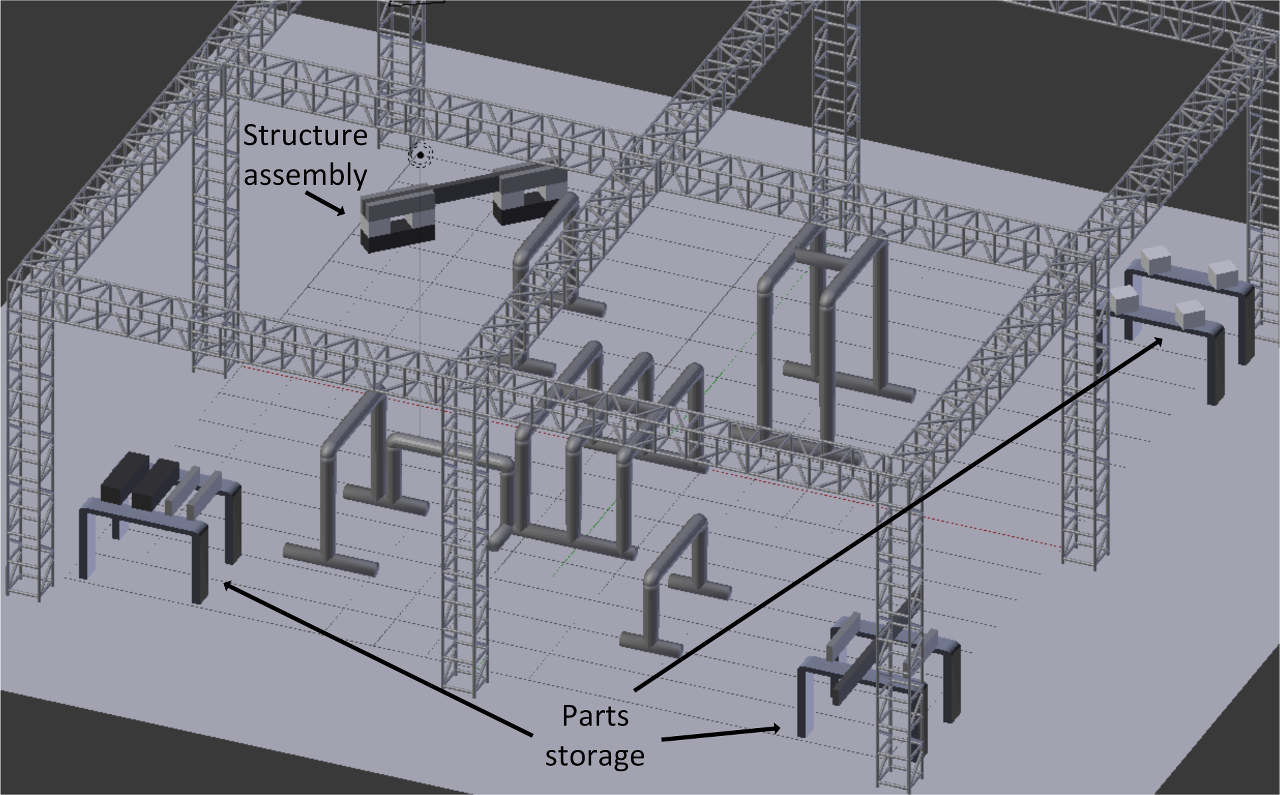
\includegraphics[width=1.0\columnwidth]{environment_visio.png}
    \caption[Environment modelled for the mission.]{Environment modelled for the mission. The parts are initially stored in three different stock areas and finally assembled in the top left area of this figure.}
    \label{fig:environment}
\end{figure}

\begin{figure}
    \centering
    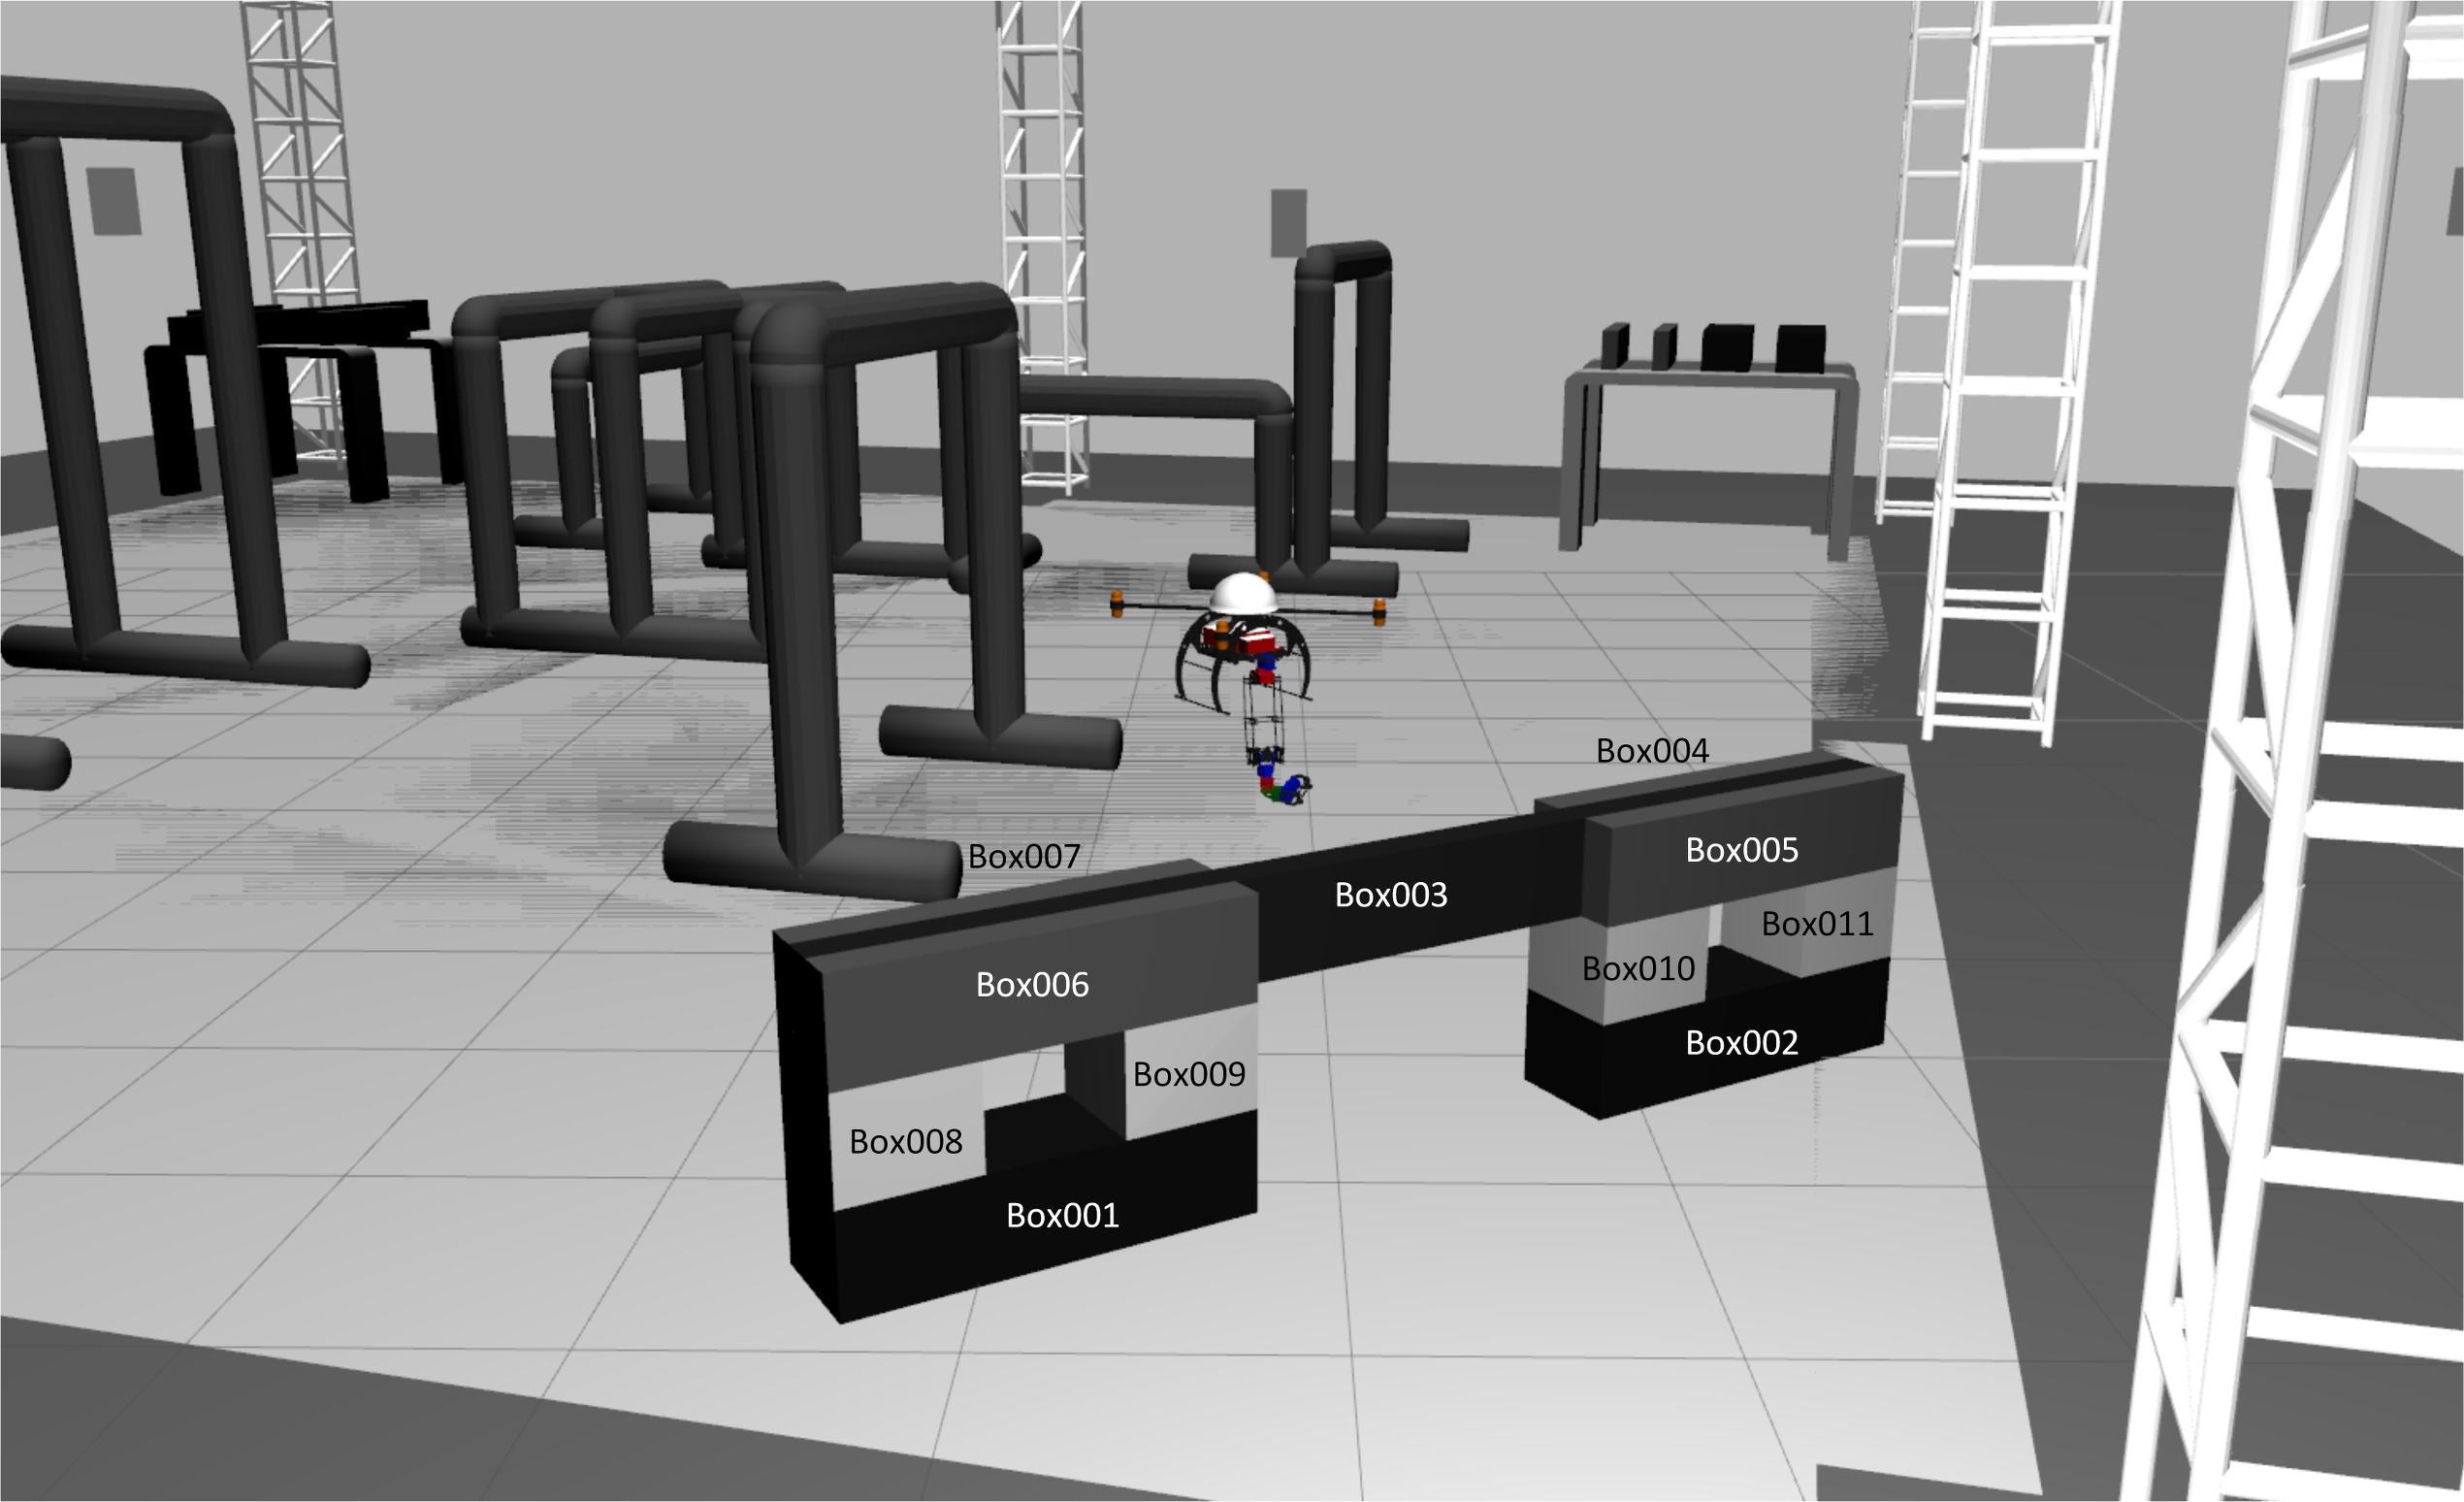
\includegraphics[width=1.0\columnwidth]{structure_visio.png}
    \caption[Structure to assemble for the mission.]{Structure to assemble for the mission. The structure is composed of eleven parts, enumerated from Box001 to Box011. All the parts are supposed to have a flat handle from which the robotic arms of the UAS can pick them.}
    \label{fig:structure}
\end{figure}

The entry point to the system is the 3D CAD environment model that contains the initial state (stock parts and home locations of the UAS) and the 3D CAD model of the structure to be built. The assembly planner reads the 3D CAD model of the structure and generates a valid assembly plan. Each of the assembly tasks contain two nodes: one with the \textit{effect} of the operation and one with the \textit{preconditions} for the operation. The effect of the operation is the part that will be assembled after the task execution, whereas the preconditions for the operation are the parts that must be assembled prior to the execution of the task. Part of the assembly plan generated by the assembly planner is shown in Listing~\ref{AssemblyPlan}.

\lstinputlisting[label=AssemblyPlan,caption=First tasks of the assembly plan generated by the assembly planner. The tasks are partially ordered meaning that a single UAS could do the assembly correctly by executing the tasks in that order. However tasks that appear later in the file may be executed before some of the previous as is the case of the part Box001 which constitutes a base part and thus do not depend on any other.]{AssemblyPlan.xml}

%The task allocation planner reads the assembly plan and generates and assignment problem with the definition of the following entities:
%
%\begin{itemize}
%  \item Locations: the different points of the environment where the parts are initially located or where the tasks have to be executed.
%  \item Starting points: the home locations of the UAS.
%  \item UAS: the available vehicles to perform the mission with their associated home locations and the maximum load capacity.
%  \item Tasks: the tasks of the mission with their part name, parts weight, part initial location and assembly location.
%\end{itemize}

As it has been previously commented in Section~\ref{sec:ddesc}, in order to exploit the capabilities of a team with multiple UAS, at the allocation planner level, tasks can be decomposed to be shared among different UAS. That is the case of the assembly tasks associated to Box001, Box002 and Box003 whose weight of 900 grams is higher than the payload of a single UAS. The task for each of these parts is automatically decomposed into two different tasks of 450 grams. 

%(see Listing~\ref{ArcasAssemblyProblem}). 
%
%\lstinputlisting[label=ArcasAssemblyProblem,caption=Task discretization generated by the allocation planner for some tasks whose parts have the highest weight values. The tasks for the parts that have a weight value of 900 grams have been discretized into two different tasks with same ID but half the original weight value. Tasks with an empty precondition list do not depends on others and could be executed at any time. The order on which the tasks appear in the assignment problem file is not relevant.]{ArcasAssemblyProblem.xml}

The task allocation planner solves the assignment problem and in the solution it can be seen that the parts are assigned to their closer vehicles, and the three parts with higher weight are shared between two UAS. The solver was configured to apply two phases: a Construction Heuristic and a Metaheuristic. The Construction Heuristic chosen was the so called First Fit Decreasing, which assigns the more difficult planning entities first (those tasks with a higher part weight in our case), so it sorts the planning entities on decreasing difficulty. The Metaheuristic chosen was the Late Acceptance, a variant of the Hill Climbing local search. Late Acceptance does, for the assignment initially computed by the Construction Heuristic, some moves between the planning entities, one per iteration, and accepts any move that leads to a score that is better than the best score of a number of moves ago. This allows to do one move that initially leads to a worse score than the previous to improve the score calculated some moves ago. 

After the initial assignment problem has been solved, the task allocation planner generates a planning problem in a format suitable for the symbolic planner based on JSHOP2. This JSHOP2 planning problem contains the high level task that represent the whole structure assembly and that should be decomposed into primitives, as well as the initial states of all the entities involved. Listing~\ref{JSHOP2Problem} shows the planning problem generated for our mission containing, among others, the assignment from parts to UAS generated by the task allocation planner and the dependencies computed for each of the parts by the assembly planner. 

\lstinputlisting[label=JSHOP2Problem,caption=JSHOP2 planning problem.]{problem.txt}

The plan computed by the symbolic planner contains all the primitives for each of the UAS involved in the mission execution and it has been represented with a Gantt chart in Fig.~\ref{fig:gantt}. The symbolic planner produced a schedule of all the assembly tasks computed by the assembly planner. In the cases where multiple choices could be done, the planner decided to assemble first those parts that were dependencies for other parts that could not be assembled yet. That produced for the assignment computed by the task allocation planner the optimal scheduling of the assembly tasks.

\begin{figure*}
    \centering
    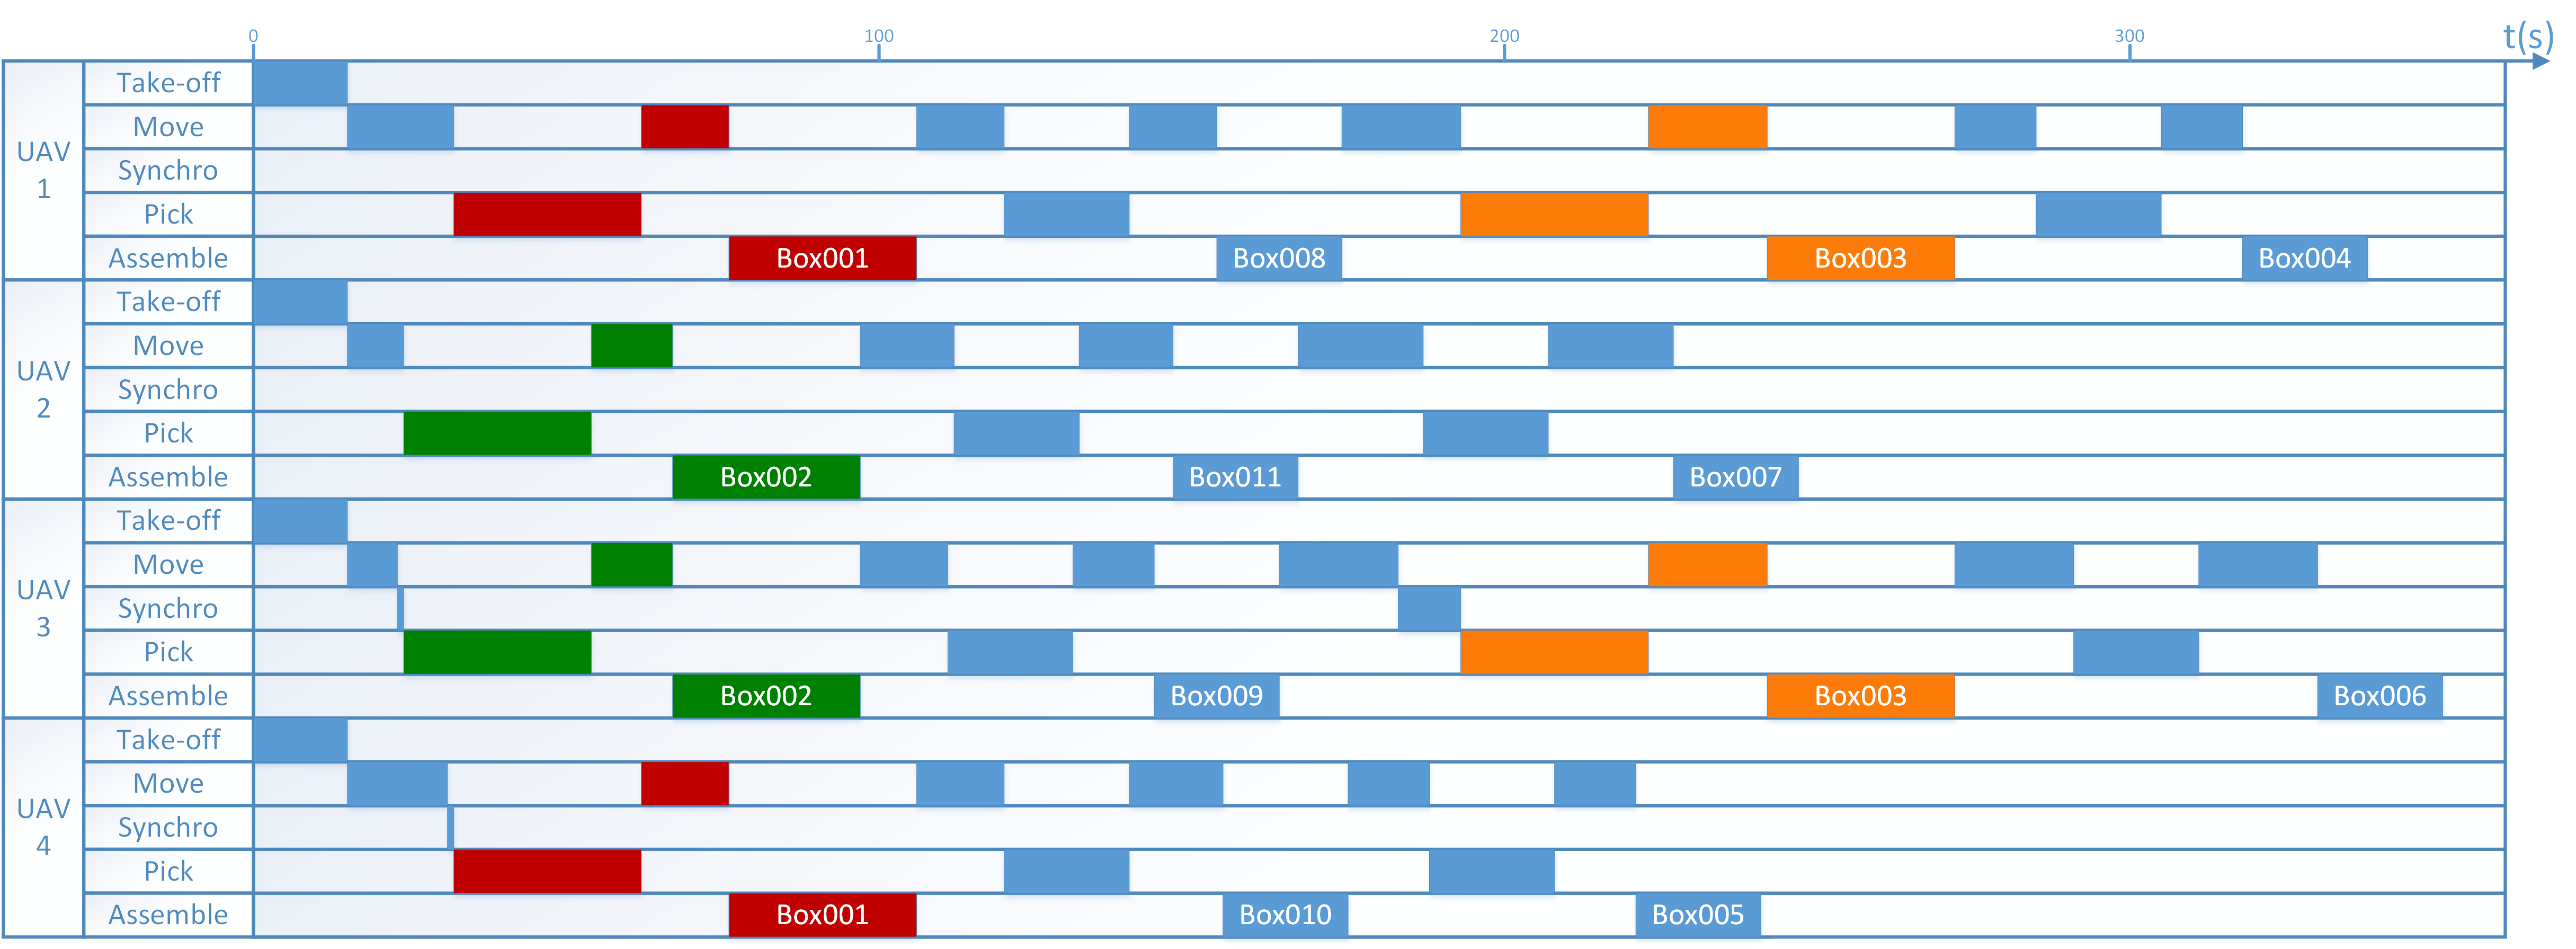
\includegraphics[width=0.99\textwidth]{gantt.png}
    \caption[Gantt chart of the final plans computed by the task planner.]{Gantt chart of the final plan computed by the symbolic planner. Each rectangle represents a primitive task. Primitives with a string on top represent the assembly task of the part with the given name. Primitives of blue color are independent and are executed by the vehicles individually. Primitives of red, green and orange color are cooperatives and thus are executed by the UAS on which they appear simultaneously. Cooperative primitives appear on parts that must be managed by two UAS simultaneously due to their weight. Red primitives are executed cooperatively and simultaneosly by UAV1 and UAV4 in order to assemble the part Box001, green primitives by UAV2 and UAV3 to assemble Box002 and orange primitives by UAV1 and UAV3 to assemble Box003.}
    \label{fig:gantt}
\end{figure*}

\section{Conclusions and Future Work}
	\label{sec:conclusions}

The main contribution of this paper is the implementation of an assembly planner capable of generating assembly plans doing stability checks during the planning process, taking into account external forces such as the gravity. The system developed performs task assignment and ordering given the number of UAS in order to maximize the parallelism and cooperation in the mission. 

The current system computes the optimal scheduling of the assembly tasks computed by the assembly planner given the assignment produced by the task allocation planner. Future work will explore an integrated optimal scheduling combining both task allocation and temporal task sequencing. In addition, as the forces generated by the UAS can have an impact in some cases in the stability of the structure, they will be added in the simulation stage of the assembly planner.

Finally the approach has been tested in missions involving multiple simulated UAS. In future work the goal is to execute the mission with real UAS in order to find more realistic and complex contexts to test the architecture developed.

%-----------------------------------------------------------------------------
% BIBLIOGRAPHY
%-----------------------------------------------------------------------------
\bibliographystyle{IEEEtran}
\bibliography{IEEEabrv,bibliography}

\end{document}